\chapter{Fundamentos de la minería de texto}
En este capítulo discutiremos algunas de las técnicas y términos más importantes a la hora de hablar de minería de texto, así como minería de datos en general, con objeto de que todas las consideraciones realizadas posteriormente queden claras.

En \textit{Text Mining Applied to Electronic Medical Records: A Literature Review}~\cite{textmining2015} se hace una revisión de los diferentes aspectos a tener en cuenta durante el procesamiento de textos médicos. Nos apoyaremos en gran medida en la estructura, contenidos y referencias de este artículo, que resume muy bien todo lo que necesitamos saber para resolver nuestro problema.

\section{Minería de datos}
La minería de datos es una rama de la informática que se dedica a encontrar tendencias y patrones en grandes volúmenes de información. Estas tendencias y patrones crean \textit{conocimiento} a partir de los datos, es decir: información estructurada desde los datos no estructurados. Esta información es muy valiosa y contribuye en las decisiones que se vayan a tomar o a monitorizar algunos aspectos que sean de vital importancia para el interesado. 

La minería de datos puede dividirse en un número de técnicas que funcionan de forma diferente en función del tipo de datos que tengamos y la información que busquemos.

\begin{enumerate}
    \item \textbf{Asociación}: esta técnica se centra en encontrar relaciones entre las distintas variables de nuestros datos, con objeto de encontrar muestras que sean estadísticamente dependientes. Una de las técnicas más utilizadas son las reglas de asociación, cuya salida tras el cálculo son un conjunto de reglas con antecedentes y consecuentes, muy fácilmente interpretables por cualquier persona, familiarizada o no con la ciencia de datos. \cite{associationrules1991}
    \item \textbf{Clasificación}: el proceso de clasificación trata de asignar una categoría a un conjunto de elementos que tengan algún aspecto en común. La clasificación en la minería de datos es una de las técnicas más utilizadas, ya que la naturaleza de gran parte de los datos responden bien a este método. \cite{Kumar2012ClassificationAF}
    \item \textbf{Agrupamiento}: también denominado \textit{clustering} trata de agrupar muestras que tengan características similares. A diferencia de la clasificación, aquí no tenemos una etiqueta o categoría a la que asignar las muestras, sino que las agrupamos \textit{a ciegas}, simplemente basándonos en alguna métrica para evaluar la distancia que haya entre un determinado par de muestras. \cite{Jain1999DataCA}
    \item \textbf{Predicción}: la predicción nos ayuda a encontrar tendencias entre variables, generalmente en datos con una componente temporal fuerte. \cite{han2012mining} Es común poder predecir si un paciente sufrirá una determinada enfermedad conociendo su historial médico, por ejemplo.
    \item \textbf{Identificación de patrones secuenciales}: Al igual que la predicción, se trabaja sobre datos con una componente temporal marcada. En este caso, se buscan patrones, es decir, conjuntos o cadenas de muestras que aparecen de forma frecuente en un orden concreto.
\end{enumerate}


\section{Minería de texto}
En esta sección, discutiremos los diferentes aspectos a tener en cuenta en la minería de textos en concreto, tras haber abordado el concepto de minería de datos en un ámbito más general.


\subsection{Términos}
Definiremos algunos de los términos más utilizados en esta disciplina, guiándonos principalmente por el trabajo de Kamran Kowsari, \textit{Text Classification Algorithms: A Survey}~\cite{Kowsari2019TextCA}.

\subsubsection{Tokens}
El término más esencial en minería de textos es \textit{token}. Un token es la mínima unidad en la que dividiremos un cuerpo de texto a la hora de analizarlo. Este elemento suele corresponderse con una palabra, que en el contexto de la mayoría de los idiomas corresponde con un conjunto de letras separado por espacios anterior y posteriormente. Esto da lugar a la creación de \textit{Tokenizers}, algoritmos que toman un cuerpo de texto como una cadena de caracteres muy larga, y devuelven un vector de palabras. Estos \textit{tokenizers } no han de tomar el espacio en blanco necesariamente ni exclusivamente como criterio divisor, aunque suele ser lo más común. Algunos de los \textit{tokenizers} más famosos son:

\begin{itemize}
    
    \item \textbf{Tokenizers de palabras}
    \begin{itemize}
        \item \textbf{Standard Tokenizer}: El Standard Tokenizer divide el texto en términos siguiendo los límites de las palabras según están definidos en el algoritmo \textit{Unicode Text Segmentation}. 
        \item \textbf{Letter Tokenizer}: Divide el texto en términos cada vez que encuentra un carácter que no es una letra.
        \item \textbf{Whitespace Tokenizer}: Toma como criterio divisor el espacio en blanco.
        \item \textbf{Language Tokenizer}: Otros tipos de tokenizers adaptados a diferentes idiomas, como el inglés, que es el idioma más estudiado con diferencia, pero también otros idiomas con caracteres y reglas diferentes a aquellos basados en reglas occidentales, como el tailandés o el chino.
    \end{itemize}
    \item \textbf{Tokenizers de palabras parciales}
    \begin{itemize}
        \item \textbf{N-Gram Tokenizer}: Este tokenizador incluye un parámetro adicional. Primero divide el texto con alguna de las reglas mencionadas anteriormente, y posteriormente, divide cada término del vector resultante en una ventana deslizante de $n$ elementos, (de ahí \textit{N-Gram}). Por ejemplo: \textit{quick fox} devolvería $[$qu, ui, ic, ck$]$, $[$fo, ox$]$, dado un $n = 2$. Estos tokenizers también pueden utilizarse a nivel de párrafo, por lo que se devolverían pares de palabras, algo que puede ser muy útil para el análisis de \textit{dichos} o expresiones.
    \end{itemize}
    \item \textbf{Tokenizers de texto estructurado}
    \begin{itemize}
        \item \textbf{Pattern Tokenizer}: este tokenizer utiliza el patrón provisto como parámetro para la división de texto, utilizando expresiones regulares.
        \item \textbf{Simple Pattern Tokenizer}: este tokenizer utiliza el patrón provisto como parámetro para la división de texto, utilizando expresiones optimizadas para el patrón dado, lo que hace que funcione generalmente más rápido pero también será más específico.
    \end{itemize}
\end{itemize}

En resumen, un tokenizer es un algoritmo que divide el texto provisto siguiendo los criterios definidos por el usuario, devolviendo un vector con los elementos del texto divididos atendiendo a dichos criterios. Es una de las herramientas esenciales en la minería de texto, ya que permite generar la mínima unidad de información a partir de la que se extraerá conocimiento.

\subsubsection{Palabras vacías}
\label{sec:stopwords}
Las palabras vacías o \textit{stopwords} son términos presentes en un idioma que sirven de apoyo para la formulación de oraciones pero que no poseen información en sí. Nos referimos a los artículos, determinantes, preposiciones, etc.

Estos términos son considerados como \textit{ruido} en el procesamiento de texto, por lo que lo más usual es disponer de un diccionario de términos vacíos y filtrar el texto original, eliminando dichos términos. De esta forma, nos quedamos con las palabras más importantes. Los símbolos de puntuación también se suelen considerar como ruido; si bien son esenciales para la comprensión y estructuración de texto para los humanos, suponen un detrimento para algoritmos de clasificación.

Sin embargo, esta operación es delicada y no siempre ofrecerá buenos resultados. Por ejemplo, si tratamos de inferir la intención de la oración \textit{No me gusta el fútbol} y pasamos previamente un filtro de palabras vacías, el texto resultante sería \textit{gusta fútbol}. Dados estos términos, se infiere que se está opinando de forma positiva acerca del tema \textit{fútbol}, cuando no es así.

Este caso particular está descrito en la literatura como \textit{negation handling}, en trabajos como \cite{Farooq2017NegationHI} o \cite{Ali2020ConventionalAS}. Aún así, hay muchos factores que se deben tener en cuenta antes de eliminar términos de una oración.



\subsubsection{Stemming y Lematización}
Stemming hace referencia a la gestión de palabras con prefijos o sufijos para su integración en una frase, como plurales (casa, casa\textbf{s}). Se trata de eliminar los posibles complementos añadidos con objeto de normalizar las palabras y que todas tengan la misma forma. En este caso también han de tenerse en cuenta las negaciones (típico, \textbf{a}típico).

La lematización va un paso más allá y trata de encontrar la raíz de las palabras, obteniendo una normalización más estricta. Un buen ejemplo son la conjugación de los verbos: de \textit{estudiando}, \textit{estudiante} o \textit{estudio} obtenemos \textit{estudi-}. \cite{Lemmatization2014} 


\subsubsection{Frecuencias: TF, IDF}
Uno de los datos más importantes a obtener de un texto es la frecuencia de palabras. Esta operación es tan simple como suena: contar cuántas veces aparece cada palabra y anotarlo en una estructura similar a un diccionario. Este término se conoce como \textit{Term Frequency} o TF. Estos valores suelen representarse en una escala logarítmica, con objeto de que las palabras muy dominantes no eclipsen a las menos frecuentes.

Del campo de teoría de la información \cite{information2001} conocemos que aquellos términos que aparezcan con una frecuencia muy alta poseerán menos información que aquellos que aparezcan menos. Como vimos en la sección \ref{sec:stopwords}, eliminamos las palabras vacías porque aparecían mucho. Es decir, un artículo como \textit{el} o una preposición como \textit{de} tendrían una frecuencia desproporcionada, cuando en realidad no aportan ninguna información. 


De forma similar, el valor \textit{Inverse Document Frequency}~\cite{Jones2004ASI} trata de abarcar esta frecuencia pero en un conjunto de documentos, añadiendo la inversa de la frecuencia por documento. Esta métrica se utiliza mucho en conjunción con la TF, resultando en la TF-IDF, que trata de medir la relevancia de un término en un conjunto de documentos. Esto resulta en el cálculo:

\begin{equation}
    W(d, t) = TF(d, t) * log(\frac{N}{df(t)})
\end{equation}

donde $d$ es un documento del conjunto de documentos con cardinalidad $N$, $t$ es el término en concreto y $df(t)$ es el número de documentos que contienen el término $t$.


\subsubsection{Bolsas de palabras}
Conociendo el concepto de frecuencias de palabaras, una de las aplicaciones directas son las bolsas de palabras, que recogen en una estructura con forma de diccionario cada término y su frecuencia.

De esta forma, tenemos un \textit{ranking} para cada término. Esto se utiliza extensivamente en sistemas de recomendación, en donde una consulta provista por un usuario se compara con la bolsa de palabras del posible conjunto de documentos, y este conjunto va afinándose conforme se van comparando los conjuntos de palabras. El resultado es una búsqueda más refinada que devuelve documentos más relevantes con respecto a la consulta realizada.

\subsubsection{Word Clouds}
Las nubes de palabras o \textit{Word Clouds} son un tipo de visualización especializada en conjuntos de datos de texto. Consisten en representar el conjunto de palabras más relevantes del texto que analicemos, disponiendo dicho conjunto de forma distrubida por la imagen. Por lo general, se suelen utilizar códigos de color o tamaño para aludir a factores como la frecuencia o la relevancia de dicha palabra en el texto.

Dada una bolsa de palabras, podemos tomar los $n$ términos más presentes y escribirlos en una imagen, haciendo la fuente tanto más grande cuanto más aparezca dicha palabra. Esto ofrece una manera rápida e intuitiva de averiguar el tema del cuerpo del texto y sus términos más relevantes.


\subsection{Técnicas}
En esta sección discutiremos algunas de las técnicas avanzadas más utilizadas en procesamiento y análisis de texto que además utilizaremos en nuestra implementación directa o indirectamente.

\subsubsection{\textit{Word Embeddings}}
Esta técnica esencialmente trata de convertir los diferentes términos en vectores de números reales, ya que esto los convierte en objetos matemáticos fáciles de comparar y procesar. Matemáticamente hablando corresponde con una representación de un espacio $n$-dimensional a un espacio vectorial continuo de menor tamaño, donde $n$ es el número total de términos presentes en todos los documentos.

Esta técnica ha sido estudiada en profundidad en varios proyectos:

\begin{itemize}
    \item \textbf{Word2Vec}: esta técnica trata de representar las palabras como vectores utilizando una red neuronal con dos capas, haciendo uso de una bolsa de palabras continua (CBOW) y el modelo del Skip Gram. \cite{Mikolov2013Word2Vec}
    \item \textbf{GloVe}: acrónimo de \textit{Global Vectors for Word Representation}, es una técnica muy similar a la \textit{Word2Vec}, con la particularidad de estar preentrenada en grandes corpus de texto, basados en Wikipedia y Gigaword. \cite{Pennington2014GloveGV}
    \item \textbf{FastText}: es una técnica desarrollada por Facebook. Esta técnica hace uso de la técnica de los $n$-grams para su entrenamiento, obteniendo una representación de los términos mucho más granular. \cite{Bojanowski2017EnrichingWV}
    \item \textbf{Contextualized Word Representations}: esta técnica hace uso del contexto de las palabras para tratar de encontrar una representación y relación entre ellas. Esta técnica basa su funcionamiento en el uso de Long-Short Term Memory, un tipo de red neuronal recurrente muy utilizada en procesamiento de texto, en la que ahondaremos más en profundidad en secciones posteriores de este documento. \cite{Melamud2016context2vecLG}
\end{itemize}

\subsubsection{Reducción de dimensionalidad}
La reducción de dimensionalidad es una técnica que permite proyectar el espacio en el que se hallan nuestros datos en un subespacio de menor dimensionalidad, con objeto de facilitar el cálculo de las propiedades de dichos datos sin tener que utilizar todas sus características. Es común encontrar conjuntos de datos con un número de dimensiones muy alto, que hace inviable su estudio.

Las principales técnicas desarrolladas para reducir la dimensionalidad incluyen:

\begin{itemize}
    \item \textbf{Principal Component Analysis (PCA)}: PCA o análisis de componentes principales trata de encontrar un subespacio latente que represente a los datos encontrando aquellas variables que estén menos relacionadas y que maximicen la varianza, para conservar la mayor cantidad de variabilidad posible. \cite{Jolliffe:1986} 
    \item \textbf{Independent Component Analysis (ICA)}: es una técnica similar que trata de expresar los datos con transformaciones lineales. \cite{Hyvrinen2014TopographicIC}
    \item \textbf{Linear Discriminant Analysis (LDA)}: es otro método muy utilizado cuando los datos son de caracter categórico y no tienen una proporcion uniforme intraclase. \cite{LDA2009}
\end{itemize}

Toda esta familia de algoritmos resulta muy conveniente para \textit{comprimir} datos de alta dimensionalidad y extraer solo las \textbf{características principales} de los mismos. Se suelen usar en etapas de preprocesamiento, donde los datos resultantes se pasan a los algoritmos a entrenar, consiguiendo un mejor resultado y rendimiento en comparación con los datos sin preprocesar.

\subsubsection{Clasificación de texto}
Por último, abordaremos las principales técnicas para clasficar texto, ámbito importante en nuestro proyecto, así como una breve explicación de las mismas. Al igual que en las secciones anteriores, no es nuestro objetivo estudiarlas en profundida, pero más bien ofrecer una vista general del panorama en cuanto a esta tecnología con objeto de que el lector se familiarice con los términos.


Los principales algoritmos de clasificación de texto, entre otros, son los siguientes:

\begin{itemize}
    \item \textbf{Boosting y bagging}: boosting y bagging son dos algoritmos basados en lo que se denomina en la literatura como \textit{ensemble learning}. Esta técnica utiliza un gran número de modelos que funcionan muy bien para casos muy específicos pero no generalizan correctamente. La idea es que la respuesta conjunta de todos los modelos nos acerque a la respuesta correcta. Esta decisión puede hacerse mediante votos u otros métodos. \cite{Bauer2004AnEC}
    \item \textbf{Regresión logística}: la regresión logística es uno de los métodos de aprendizaje más simples, junto con la regresión linear. La regresión logística es una especialización de la regresión lineal, de forma que se utiliza una función logística para predecir categorías discretas, no continuas. \cite{CoxLogit1989}
    \item \textbf{Redes neuronales recurrentes}: por último, las redes neuronales recurrentes son una especialización de las redes neuronales en las que un subonjunto de las neuronas reciben su salida como una entrada, generándose ciclos de retroalimentación o \textit{feedback}. Estas redes funcionan especialmente bien con datos con patrones y componentes temporales, características especialmente destacables del lenguaje humano, así como de la música o vídeo. \cite{ZhouLSTM}
\end{itemize}


Existen otras muchas técnicas en clasificación de texto, como \textit{K Nearest Neighbours}~\cite{KNNXiao2007}, \textit{Naïve Bayes}~\cite{FrankNaive2006}, \textit{Support Vector Machines (SVM)}~\cite{SVMJoa1998}, árboles de decisión~\cite{DecisionTreeNoorman2018} o \textit{Random Forests}~\cite{breiman2001random}, entre muchas otras. 

\section{Estado del arte}

Por último, mencionaremos brevemente los tres proyectos más grandes de lenguaje generativo hasta la fecha, con objeto de entender qué es lo que hacen para poder integrar dichas técnicas en nuestro modelo.

\subsection{Transformers}
En esta sección hablaremos del Transformer, un tipo de arquitectura de red neuronal creada por ingenieros de Google \cite{TransformerAshish2017}, en más profundidad, sus características principales en contraste con las demás tecnologías y de la configuración escogida para nuestro problema.

\subsubsection{Arquitectura y módulos de atención}
El Transformer corresponde con una de las técnicas más modernas de procesamiento de lenguaje natural, y una de las más relevantes del momento. Se la presenta como \textit{estado del arte en procesamiento del lenguaje natural}, constituyendo un modelo mucho más potente y \textbf{considerado} que las anteriores LSTM.

El transformer está princpalmente basado en redes recurrentes, redes cuya entrada está conectada a la salida y, generalmente, se las construye con un contexto temporal en mente. Esto quiere decir que dada una entrada en el momento $n$, predeciremos la salida en función de la salida que se obtuvo en el momento $n - 1$, además de la entrada del momento $n$ en sí.

Esto es en sí el funcionamiento de una red recurrente estándar. El transformer añade varios conceptos clave a su implementación que lo hacen particularmente poderoso que serán detallados a continuación.

\begin{figure}[h]
    \centering
    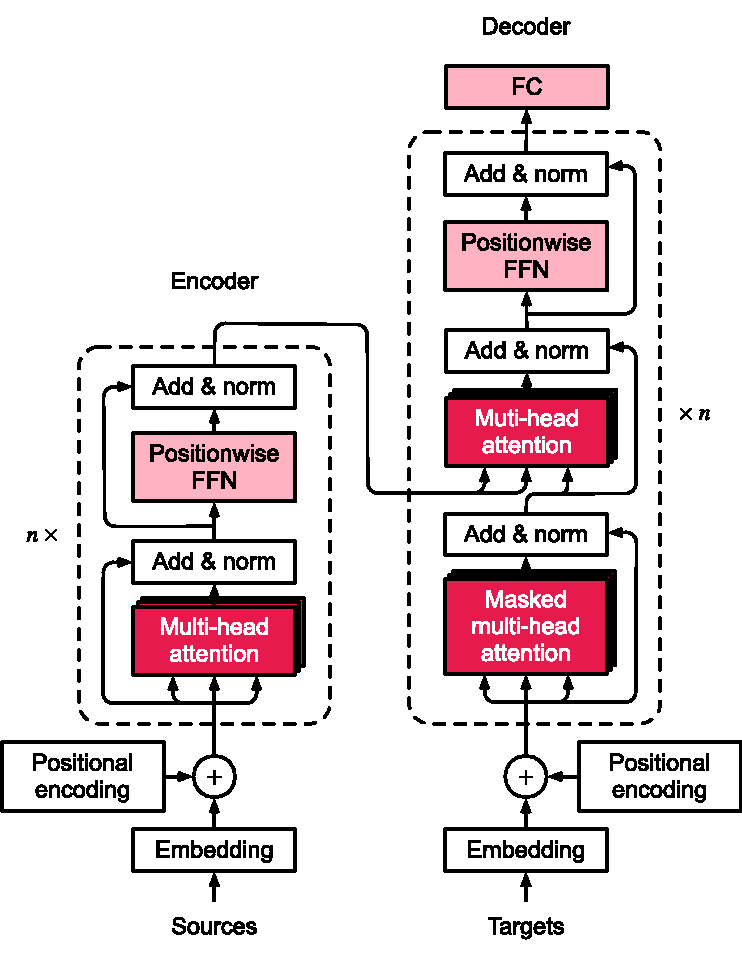
\includegraphics[width=.5\textwidth]{media/transformer.pdf}
    \caption{Diagrama de un transformer [extraído de \cite{TransformerAshish2017}]}
    \label{fig:transformer}
\end{figure}

\subsubsection{Atención}
Uno de los principales conceptos que añade el transformer es de la \textbf{atención}. Este concepto trata de emular el concepto de atención con el que todos estamos familiarizados: el de ponderar y distrubir los recursos cognitivos de forma que aquellos estímulos más importantes reciban más recursos de cómputo por parte del sistema, de la misma forma que nuestro cerebro procesa de forma más potente aquello en lo que estamos concentrados, ignorando aquellos estímulos que sean menos importantes en un determinado instante.

Uno de los principales problemas de las redes neuronales recurrentes clásicas es ls imposibilidad de la paralelización de su ejecución, y el crecimiento de los términos a considerar conforme más avanzado es el análisis de la secuencia en concreto.

La técnica de \textit{multi-head attention}, que podemos apreciar en color en la Figura \ref{fig:transformer}, soluciona estos problemas. En primer lugar, hace la paralelización del modelo no solo posible, sino también muy fácil. Cada módulo calcula por separado la atención que le corresponda y posteriormente se concatenan y se transforman linealmente en la salida de la dimensión que se espera. 

Por otro lado, los modelos tradicionales sufren de no considerar dependencias entre elementos si estos están distantes en la secuencia. Los diferentes módulos calculan la atención en diferentes puntos de la secuencia de forma paralela, como comentamos. Las diferentes zonas pueden efectivamente considerar zonas muy distantes en tiempo constante, gracias a la paralelización. Esto efectivamente soluciona el problema de olvidar características importantes de puntos distantes, así como evitando tener que crear caminos de cálculo cada vez más largos conforme avanzamos en el análisis de la secuencia.


\subsection{Modelos basados en transformers}
Habiendo descrito brevemente la arquitectura de un transformer en general, veamos qué se ha desarrollado con esta nueva tecnología.

\subsubsection{BERT}
BERT son las siglas en inglés de \textit{Bidirectional Encoder Representations from Transformers}~\cite{bertDevlin2019}. Es un modelo de lenguaje generativo basado en un encoder bidireccional como su nombre indica. Este modelo fue uno de los primeros en realmente conseguir una fluidez comunicativa convincente. Su arquitectura preentrenada permite, con una sola capa extra, craer modelos para tareas en casi cualquier ámbito, como responder preguntas o inferencia del lenguaje, sin necesidad de modificar particularmente su arquitectura interna.


\subsubsection{LaMDA}
LaMDA corresponde con las siglas de \textit{Language Model for Dialogue Applications}~\cite{LaMDAGoogle2020}, un proyecto de Google que compite de forma directa con los modelos antes mencionados. Al igual que los dos proyectos anteriores, LaMDA está basado en un transformer, una arquitectura de redes neuronales creada también por Google~\cite{TransformerAshish2017}, que explicaremos en más profundidad en los siguientes capítulos. Este proyecto se creó con una aplicación en concreto: un \textit{chatbot} automático lo más natural posible, al que llamaron \textit{Meena}. Según las estadísticas de Google, Meena tiene casi el doble de capacidad de predicción e inferencia que el antiguo GPT-2, y se entrenó en 8 veces más datos. Es el buque insignia de la empresa.

\subsubsection{GPT-3 Open AI}
GPT son las siglas de \textit{Generative Pre-trained Transformer}~\cite{GPT3openAI2020} y 3 indica la versión. Este modelo trata de abarcar los problemas que otros transformers solían tener, como es la habilidad de un humano para continuar una tarea lingüística dado muy poco contexto o instrucciones. Escalando los modelos se logra mejorar significativamente la generalización del mismo y se descubre que no es necesario afinar los parámetros de los modelos, sino que esto puede corresponderse más con un problema de meta-aprendizaje.

Existen varias versiones del GPT-3, entrenadas en diferentes tamaños, desde 125 millones en la versión que denominan pequeña, hasta 175 mil millones, que es la versión que los investigadores denominan como ``GPT-3'' a secas. Jared Kaplan sugiere en \cite{kaplan2020scaling} que la función de pérdida en la etapa de validación debería corresponderse con la ley de potencia, (también conocida como el principio de Pareto) en función del tamaño de dicha red, de ahí que se probaran distintas configuraciones y tamaños.

Para nuestro proyecto, hemos escogido el modelo GPT-2, de OpenAI. Concretamente usaremos la versión pequeña, que consta de 117M de parámetros. Este modelo fue entrenado en una base de datos de texto tomada de Wikipedia, constando de más de 60GB de datos de texto. 

Utilizaremos el modelo preentrenado, que ya de por sí es capaz de hablar de forma genérica, y lo entrenaremos con nuestra base de datos para que aprenda a hablar tal y como lo haría un médico.



